\documentclass[11pt]{article}
\usepackage[a4paper,margin=2.5cm]{geometry}
\usepackage[T1]{fontenc}
\usepackage[utf8]{inputenc}
\usepackage{lmodern}
\usepackage{amsmath,amssymb}
\usepackage{booktabs}
\usepackage{graphicx}
\usepackage{xcolor}
\usepackage[numbers,sort&compress]{natbib}
\usepackage[colorlinks=true,linkcolor=blue!50!black,citecolor=blue!50!black,urlcolor=blue!50!black,pdftitle={Jumps or Asymmetric Tails? Levy Jump-Diffusion Models and the Tail Risk of the Mexican Peso},pdfauthor={Michele Ferraz Figueiro}]{hyperref}
\usepackage{setspace}
\usepackage{seqsplit} % lets the long SHA-256 checksum break across lines
\usepackage{caption}
\captionsetup{font=small,labelfont=bf}
\setstretch{1.15}

% Auto-generated by mxntail.reporting. Do not edit.
\newcommand{\appEsGarchKou}{343.2}
\newcommand{\appEsGarchMerton}{337.4}
\newcommand{\appEsGarchSkewT}{356.6}
\newcommand{\appEsGarchT}{329.1}
\newcommand{\appEsGaussian}{293.1}
\newcommand{\appEsKou}{422.9}
\newcommand{\appEsMerton}{419.6}
\newcommand{\appEsStudentT}{417.8}
\newcommand{\appShortGarchKou}{3,671}
\newcommand{\appShortGarchMerton}{3,794}
\newcommand{\appShortGarchSkewT}{2,776}
\newcommand{\appShortGarchT}{3,351}
\newcommand{\appShortGaussian}{12,096}
\newcommand{\appShortKou}{6,194}
\newcommand{\appShortMerton}{6,268}
\newcommand{\appShortStudentT}{6,996}
\newcommand{\dmpFzNineFiveGarchKou}{0.953}
\newcommand{\dmpFzNineFiveGarchMerton}{0.858}
\newcommand{\dmpFzNineFiveGarchSkewT}{0.009}
\newcommand{\dmpFzNineFiveGaussian}{0.002}
\newcommand{\dmpFzNineFiveKou}{$<$0.001}
\newcommand{\dmpFzNineFiveMerton}{$<$0.001}
\newcommand{\dmpFzNineFiveStudentT}{$<$0.001}
\newcommand{\dmpFzNineNineGarchKou}{0.380}
\newcommand{\dmpFzNineNineGarchMerton}{0.287}
\newcommand{\dmpFzNineNineGarchSkewT}{0.062}
\newcommand{\dmpFzNineNineGaussian}{0.011}
\newcommand{\dmpFzNineNineKou}{0.010}
\newcommand{\dmpFzNineNineMerton}{0.011}
\newcommand{\dmpFzNineNineStudentT}{0.015}
\newcommand{\dmpNlsGarchKou}{0.318}
\newcommand{\dmpNlsGarchMerton}{0.197}
\newcommand{\dmpNlsGarchSkewT}{0.004}
\newcommand{\dmpNlsGaussian}{0.003}
\newcommand{\dmpNlsKou}{$<$0.001}
\newcommand{\dmpNlsMerton}{$<$0.001}
\newcommand{\dmpNlsStudentT}{$<$0.001}
\newcommand{\dmtFzNineFiveGarchKou}{-0.06}
\newcommand{\dmtFzNineFiveGarchMerton}{-0.18}
\newcommand{\dmtFzNineFiveGarchSkewT}{-2.60}
\newcommand{\dmtFzNineFiveGaussian}{3.05}
\newcommand{\dmtFzNineFiveKou}{3.40}
\newcommand{\dmtFzNineFiveMerton}{3.45}
\newcommand{\dmtFzNineFiveStudentT}{3.30}
\newcommand{\dmtFzNineNineGarchKou}{0.88}
\newcommand{\dmtFzNineNineGarchMerton}{1.06}
\newcommand{\dmtFzNineNineGarchSkewT}{-1.87}
\newcommand{\dmtFzNineNineGaussian}{2.55}
\newcommand{\dmtFzNineNineKou}{2.58}
\newcommand{\dmtFzNineNineMerton}{2.55}
\newcommand{\dmtFzNineNineStudentT}{2.42}
\newcommand{\dmtNlsGarchKou}{1.00}
\newcommand{\dmtNlsGarchMerton}{1.29}
\newcommand{\dmtNlsGarchSkewT}{-2.91}
\newcommand{\dmtNlsGaussian}{2.94}
\newcommand{\dmtNlsKou}{5.20}
\newcommand{\dmtNlsMerton}{4.49}
\newcommand{\dmtNlsStudentT}{6.37}
\newcommand{\excNFGarchKou}{360}
\newcommand{\excNFGarchMerton}{369}
\newcommand{\excNFGarchSkewT}{338}
\newcommand{\excNFGarchT}{406}
\newcommand{\excNFGaussian}{311}
\newcommand{\excNFKou}{346}
\newcommand{\excNFMerton}{345}
\newcommand{\excNFStudentT}{416}
\newcommand{\excNNGarchKou}{73}
\newcommand{\excNNGarchMerton}{78}
\newcommand{\excNNGarchSkewT}{74}
\newcommand{\excNNGarchT}{96}
\newcommand{\excNNGaussian}{123}
\newcommand{\excNNKou}{55}
\newcommand{\excNNMerton}{54}
\newcommand{\excNNStudentT}{90}
\newcommand{\expExcNNGarchKou}{72}
\newcommand{\expExcNNGarchMerton}{70}
\newcommand{\expExcNNGarchSkewT}{68}
\newcommand{\expExcNNGarchT}{97}
\newcommand{\expExcNNGaussian}{45}
\newcommand{\expExcNNKou}{23}
\newcommand{\expExcNNMerton}{16}
\newcommand{\expExcNNStudentT}{51}
\newcommand{\expNinetyFive}{311}
\newcommand{\expNinetyNine}{62}
\newcommand{\expNlsGarchKou}{0.9116}
\newcommand{\expNlsGarchMerton}{0.9130}
\newcommand{\expNlsGarchSkewT}{0.9060}
\newcommand{\expNlsGarchT}{0.9113}
\newcommand{\expNlsGaussian}{1.1826}
\newcommand{\expNlsKou}{1.0071}
\newcommand{\expNlsMerton}{1.0145}
\newcommand{\expNlsStudentT}{0.9966}
\newcommand{\gapShare}{22}
\newcommand{\gkMeanDn}{0.46}
\newcommand{\gkMeanUp}{0.46}
\newcommand{\gkPup}{0.84}
\newcommand{\gkQ}{0.223}
\newcommand{\gmDeltaJ}{0.706}
\newcommand{\gmJumpEvery}{7}
\newcommand{\gmLambda}{0.135}
\newcommand{\gmMuJ}{0.304}
\newcommand{\gsLam}{0.154}
\newcommand{\gsLamSe}{0.016}
\newcommand{\gsNu}{7.0}
\newcommand{\gsPersist}{0.986}
\newcommand{\gtNu}{6.6}
\newcommand{\gtPersist}{0.986}
\newcommand{\kurtFull}{107.0}
\newcommand{\kurtMain}{9.9}
\newcommand{\llGainKou}{0.4}
\newcommand{\llGainMerton}{-10.9}
\newcommand{\llGainSkew}{45.1}
\newcommand{\llGarchKou}{-6,591.5}
\newcommand{\llGarchMerton}{-6,602.7}
\newcommand{\llGarchSkewT}{-6,546.8}
\newcommand{\llGarchT}{-6,591.9}
\newcommand{\llGaussian}{-8,067.5}
\newcommand{\llKou}{-7,218.8}
\newcommand{\llLossMerton}{10.9}
\newcommand{\llMerton}{-7,246.6}
\newcommand{\llStudentT}{-7,226.3}
\newcommand{\maxFull}{20.2}
\newcommand{\maxMain}{8.11}
\newcommand{\mcBiasDeltaj}{-0.009}
\newcommand{\mcBiasLambda}{0.006}
\newcommand{\mcBiasMuj}{0.057}
\newcommand{\mcBicGarchMertonGarchKou}{0}
\newcommand{\mcBicGarchMertonGarchMerton}{86}
\newcommand{\mcBicGarchMertonGarchSkewT}{6}
\newcommand{\mcBicGarchMertonGarchT}{8}
\newcommand{\mcBicGarchMertonGaussian}{0}
\newcommand{\mcBicGarchMertonKou}{0}
\newcommand{\mcBicGarchMertonMerton}{0}
\newcommand{\mcBicGarchMertonStudentT}{0}
\newcommand{\mcBicGarchSkewTGarchKou}{0}
\newcommand{\mcBicGarchSkewTGarchMerton}{1}
\newcommand{\mcBicGarchSkewTGarchSkewT}{90}
\newcommand{\mcBicGarchSkewTGarchT}{9}
\newcommand{\mcBicGarchSkewTGaussian}{0}
\newcommand{\mcBicGarchSkewTKou}{0}
\newcommand{\mcBicGarchSkewTMerton}{0}
\newcommand{\mcBicGarchSkewTStudentT}{0}
\newcommand{\mcBicGarchTGarchKou}{0}
\newcommand{\mcBicGarchTGarchMerton}{0}
\newcommand{\mcBicGarchTGarchSkewT}{2}
\newcommand{\mcBicGarchTGarchT}{98}
\newcommand{\mcBicGarchTGaussian}{0}
\newcommand{\mcBicGarchTKou}{0}
\newcommand{\mcBicGarchTMerton}{0}
\newcommand{\mcBicGarchTStudentT}{0}
\newcommand{\mcBicGaussianGarchKou}{0}
\newcommand{\mcBicGaussianGarchMerton}{0}
\newcommand{\mcBicGaussianGarchSkewT}{0}
\newcommand{\mcBicGaussianGarchT}{0}
\newcommand{\mcBicGaussianGaussian}{100}
\newcommand{\mcBicGaussianKou}{0}
\newcommand{\mcBicGaussianMerton}{0}
\newcommand{\mcBicGaussianStudentT}{0}
\newcommand{\mcBicMertonGarchKou}{0}
\newcommand{\mcBicMertonGarchMerton}{0}
\newcommand{\mcBicMertonGarchSkewT}{0}
\newcommand{\mcBicMertonGarchT}{0}
\newcommand{\mcBicMertonGaussian}{0}
\newcommand{\mcBicMertonKou}{0}
\newcommand{\mcBicMertonMerton}{80}
\newcommand{\mcBicMertonStudentT}{20}
\newcommand{\mcDiffGarchMertonGarchKou}{-0.0002}
\newcommand{\mcDiffGarchMertonGarchMerton}{0.0000}
\newcommand{\mcDiffGarchMertonGarchSkewT}{0.0045}
\newcommand{\mcDiffGarchMertonGarchT}{0.0067}
\newcommand{\mcDiffGarchMertonGaussian}{0.1252}
\newcommand{\mcDiffGarchMertonKou}{0.0766}
\newcommand{\mcDiffGarchMertonMerton}{0.0766}
\newcommand{\mcDiffGarchMertonStudentT}{0.0778}
\newcommand{\mcDiffGarchSkewTGarchKou}{0.0085}
\newcommand{\mcDiffGarchSkewTGarchMerton}{0.0107}
\newcommand{\mcDiffGarchSkewTGarchSkewT}{0.0000}
\newcommand{\mcDiffGarchSkewTGarchT}{0.0060}
\newcommand{\mcDiffGarchSkewTGaussian}{0.3170}
\newcommand{\mcDiffGarchSkewTKou}{0.1220}
\newcommand{\mcDiffGarchSkewTMerton}{0.1320}
\newcommand{\mcDiffGarchSkewTStudentT}{0.1174}
\newcommand{\mcDiffGarchTGarchKou}{0.0071}
\newcommand{\mcDiffGarchTGarchMerton}{0.0078}
\newcommand{\mcDiffGarchTGarchSkewT}{0.0004}
\newcommand{\mcDiffGarchTGarchT}{0.0000}
\newcommand{\mcDiffGarchTGaussian}{0.3064}
\newcommand{\mcDiffGarchTKou}{0.1186}
\newcommand{\mcDiffGarchTMerton}{0.1259}
\newcommand{\mcDiffGarchTStudentT}{0.1122}
\newcommand{\mcDiffGaussianGarchKou}{0.0004}
\newcommand{\mcDiffGaussianGarchMerton}{0.0005}
\newcommand{\mcDiffGaussianGarchSkewT}{0.0007}
\newcommand{\mcDiffGaussianGarchT}{0.0003}
\newcommand{\mcDiffGaussianGaussian}{0.0000}
\newcommand{\mcDiffGaussianKou}{0.0002}
\newcommand{\mcDiffGaussianMerton}{0.0004}
\newcommand{\mcDiffGaussianStudentT}{0.0001}
\newcommand{\mcDiffMertonGarchKou}{0.0006}
\newcommand{\mcDiffMertonGarchMerton}{0.0002}
\newcommand{\mcDiffMertonGarchSkewT}{0.0032}
\newcommand{\mcDiffMertonGarchT}{0.0057}
\newcommand{\mcDiffMertonGaussian}{0.0812}
\newcommand{\mcDiffMertonKou}{0.0004}
\newcommand{\mcDiffMertonMerton}{0.0000}
\newcommand{\mcDiffMertonStudentT}{0.0054}
\newcommand{\mcExcGarchMertonGarchKou}{1.12}
\newcommand{\mcExcGarchMertonGarchMerton}{1.08}
\newcommand{\mcExcGarchMertonGarchSkewT}{1.26}
\newcommand{\mcExcGarchMertonGarchT}{1.51}
\newcommand{\mcExcGarchMertonGaussian}{2.34}
\newcommand{\mcExcGarchMertonKou}{1.15}
\newcommand{\mcExcGarchMertonMerton}{1.24}
\newcommand{\mcExcGarchMertonStudentT}{1.58}
\newcommand{\mcExcGarchSkewTGarchKou}{1.18}
\newcommand{\mcExcGarchSkewTGarchMerton}{1.23}
\newcommand{\mcExcGarchSkewTGarchSkewT}{1.04}
\newcommand{\mcExcGarchSkewTGarchT}{1.51}
\newcommand{\mcExcGarchSkewTGaussian}{2.38}
\newcommand{\mcExcGarchSkewTKou}{1.33}
\newcommand{\mcExcGarchSkewTMerton}{1.35}
\newcommand{\mcExcGarchSkewTStudentT}{1.69}
\newcommand{\mcExcGarchTGarchKou}{1.13}
\newcommand{\mcExcGarchTGarchMerton}{1.14}
\newcommand{\mcExcGarchTGarchSkewT}{1.00}
\newcommand{\mcExcGarchTGarchT}{0.98}
\newcommand{\mcExcGarchTGaussian}{1.96}
\newcommand{\mcExcGarchTKou}{1.19}
\newcommand{\mcExcGarchTMerton}{1.19}
\newcommand{\mcExcGarchTStudentT}{1.27}
\newcommand{\mcExcGaussianGarchKou}{1.01}
\newcommand{\mcExcGaussianGarchMerton}{1.01}
\newcommand{\mcExcGaussianGarchSkewT}{0.97}
\newcommand{\mcExcGaussianGarchT}{0.97}
\newcommand{\mcExcGaussianGaussian}{1.00}
\newcommand{\mcExcGaussianKou}{1.00}
\newcommand{\mcExcGaussianMerton}{1.00}
\newcommand{\mcExcGaussianStudentT}{0.97}
\newcommand{\mcExcMertonGarchKou}{1.00}
\newcommand{\mcExcMertonGarchMerton}{1.01}
\newcommand{\mcExcMertonGarchSkewT}{1.13}
\newcommand{\mcExcMertonGarchT}{1.54}
\newcommand{\mcExcMertonGaussian}{2.50}
\newcommand{\mcExcMertonKou}{1.00}
\newcommand{\mcExcMertonMerton}{1.01}
\newcommand{\mcExcMertonStudentT}{1.55}
\newcommand{\mcHiDeltaj}{0.915}
\newcommand{\mcHiLambda}{0.250}
\newcommand{\mcHiMuj}{0.750}
\newcommand{\mcLoDeltaj}{0.493}
\newcommand{\mcLoLambda}{0.055}
\newcommand{\mcLoMuj}{0.117}
\newcommand{\mcNlsGarchMertonGarchKou}{0.8635}
\newcommand{\mcNlsGarchMertonGarchMerton}{0.8637}
\newcommand{\mcNlsGarchMertonGarchSkewT}{0.8682}
\newcommand{\mcNlsGarchMertonGarchT}{0.8704}
\newcommand{\mcNlsGarchMertonGaussian}{0.9890}
\newcommand{\mcNlsGarchMertonKou}{0.9403}
\newcommand{\mcNlsGarchMertonMerton}{0.9403}
\newcommand{\mcNlsGarchMertonStudentT}{0.9415}
\newcommand{\mcNlsGarchSkewTGarchKou}{0.8497}
\newcommand{\mcNlsGarchSkewTGarchMerton}{0.8519}
\newcommand{\mcNlsGarchSkewTGarchSkewT}{0.8412}
\newcommand{\mcNlsGarchSkewTGarchT}{0.8472}
\newcommand{\mcNlsGarchSkewTGaussian}{1.1582}
\newcommand{\mcNlsGarchSkewTKou}{0.9632}
\newcommand{\mcNlsGarchSkewTMerton}{0.9732}
\newcommand{\mcNlsGarchSkewTStudentT}{0.9586}
\newcommand{\mcNlsGarchTGarchKou}{0.8715}
\newcommand{\mcNlsGarchTGarchMerton}{0.8721}
\newcommand{\mcNlsGarchTGarchSkewT}{0.8648}
\newcommand{\mcNlsGarchTGarchT}{0.8644}
\newcommand{\mcNlsGarchTGaussian}{1.1707}
\newcommand{\mcNlsGarchTKou}{0.9829}
\newcommand{\mcNlsGarchTMerton}{0.9902}
\newcommand{\mcNlsGarchTStudentT}{0.9765}
\newcommand{\mcNlsGaussianGarchKou}{1.0481}
\newcommand{\mcNlsGaussianGarchMerton}{1.0482}
\newcommand{\mcNlsGaussianGarchSkewT}{1.0484}
\newcommand{\mcNlsGaussianGarchT}{1.0480}
\newcommand{\mcNlsGaussianGaussian}{1.0477}
\newcommand{\mcNlsGaussianKou}{1.0479}
\newcommand{\mcNlsGaussianMerton}{1.0481}
\newcommand{\mcNlsGaussianStudentT}{1.0478}
\newcommand{\mcNlsMertonGarchKou}{0.9427}
\newcommand{\mcNlsMertonGarchMerton}{0.9423}
\newcommand{\mcNlsMertonGarchSkewT}{0.9452}
\newcommand{\mcNlsMertonGarchT}{0.9477}
\newcommand{\mcNlsMertonGaussian}{1.0232}
\newcommand{\mcNlsMertonKou}{0.9424}
\newcommand{\mcNlsMertonMerton}{0.9420}
\newcommand{\mcNlsMertonStudentT}{0.9474}
\newcommand{\mcReps}{200}
\newcommand{\mcRmseDeltaj}{0.138}
\newcommand{\mcRmseLambda}{0.073}
\newcommand{\mcRmseMuj}{0.234}
\newcommand{\mcShareGarchMertonGarchKou}{44}
\newcommand{\mcShareGarchMertonGarchMerton}{44}
\newcommand{\mcShareGarchMertonGarchSkewT}{8}
\newcommand{\mcShareGarchMertonGarchT}{4}
\newcommand{\mcShareGarchMertonGaussian}{0}
\newcommand{\mcShareGarchMertonKou}{0}
\newcommand{\mcShareGarchMertonMerton}{0}
\newcommand{\mcShareGarchMertonStudentT}{0}
\newcommand{\mcShareGarchSkewTGarchKou}{6}
\newcommand{\mcShareGarchSkewTGarchMerton}{6}
\newcommand{\mcShareGarchSkewTGarchSkewT}{77}
\newcommand{\mcShareGarchSkewTGarchT}{11}
\newcommand{\mcShareGarchSkewTGaussian}{0}
\newcommand{\mcShareGarchSkewTKou}{0}
\newcommand{\mcShareGarchSkewTMerton}{0}
\newcommand{\mcShareGarchSkewTStudentT}{0}
\newcommand{\mcShareGarchTGarchKou}{8}
\newcommand{\mcShareGarchTGarchMerton}{8}
\newcommand{\mcShareGarchTGarchSkewT}{34}
\newcommand{\mcShareGarchTGarchT}{50}
\newcommand{\mcShareGarchTGaussian}{0}
\newcommand{\mcShareGarchTKou}{0}
\newcommand{\mcShareGarchTMerton}{0}
\newcommand{\mcShareGarchTStudentT}{0}
\newcommand{\mcShareGaussianGarchKou}{10}
\newcommand{\mcShareGaussianGarchMerton}{8}
\newcommand{\mcShareGaussianGarchSkewT}{16}
\newcommand{\mcShareGaussianGarchT}{14}
\newcommand{\mcShareGaussianGaussian}{24}
\newcommand{\mcShareGaussianKou}{2}
\newcommand{\mcShareGaussianMerton}{16}
\newcommand{\mcShareGaussianStudentT}{12}
\newcommand{\mcShareMertonGarchKou}{13}
\newcommand{\mcShareMertonGarchMerton}{26}
\newcommand{\mcShareMertonGarchSkewT}{7}
\newcommand{\mcShareMertonGarchT}{3}
\newcommand{\mcShareMertonGaussian}{0}
\newcommand{\mcShareMertonKou}{16}
\newcommand{\mcShareMertonMerton}{30}
\newcommand{\mcShareMertonStudentT}{4}
\newcommand{\mcTest}{500}
\newcommand{\mcTrain}{1,500}
\newcommand{\mcTrueDeltaj}{0.706}
\newcommand{\mcTrueLambda}{0.135}
\newcommand{\mcTrueMuj}{0.304}
\newcommand{\mcsFzNineFiveGarchKou}{0.049}
\newcommand{\mcsFzNineFiveGarchMerton}{0.049}
\newcommand{\mcsFzNineFiveGarchSkewT}{1.000}
\newcommand{\mcsFzNineFiveGarchT}{0.034}
\newcommand{\mcsFzNineFiveGaussian}{0.017}
\newcommand{\mcsFzNineFiveKou}{0.012}
\newcommand{\mcsFzNineFiveMerton}{0.011}
\newcommand{\mcsFzNineFiveStudentT}{0.015}
\newcommand{\mcsFzNineNineGarchKou}{0.106}
\newcommand{\mcsFzNineNineGarchMerton}{0.106}
\newcommand{\mcsFzNineNineGarchSkewT}{1.000}
\newcommand{\mcsFzNineNineGarchT}{0.106}
\newcommand{\mcsFzNineNineGaussian}{0.080}
\newcommand{\mcsFzNineNineKou}{0.055}
\newcommand{\mcsFzNineNineMerton}{0.063}
\newcommand{\mcsFzNineNineStudentT}{0.089}
\newcommand{\mcsNlsGarchKou}{0.016}
\newcommand{\mcsNlsGarchMerton}{0.016}
\newcommand{\mcsNlsGarchSkewT}{1.000}
\newcommand{\mcsNlsGarchT}{0.016}
\newcommand{\mcsNlsGaussian}{0.016}
\newcommand{\mcsNlsKou}{0.000}
\newcommand{\mcsNlsMerton}{0.002}
\newcommand{\mcsNlsStudentT}{0.000}
\newcommand{\mcsReps}{2,000}
\newcommand{\nFull}{8,257}
\newcommand{\nMain}{7,724}
\newcommand{\nlsGarchKou}{0.9059}
\newcommand{\nlsGarchMerton}{0.9069}
\newcommand{\nlsGarchSkewT}{0.8994}
\newcommand{\nlsGarchT}{0.9036}
\newcommand{\nlsGaussian}{1.1136}
\newcommand{\nlsKou}{0.9948}
\newcommand{\nlsMerton}{1.0048}
\newcommand{\nlsStudentT}{0.9867}
\newcommand{\oosN}{6,224}
\newcommand{\oosStart}{18 December 2001}
\newcommand{\pccNNGarchKou}{0.232}
\newcommand{\pccNNGarchMerton}{0.101}
\newcommand{\pccNNGarchSkewT}{0.344}
\newcommand{\pccNNGarchT}{$<$0.001}
\newcommand{\pccNNGaussian}{$<$0.001}
\newcommand{\pccNNKou}{$<$0.001}
\newcommand{\pccNNMerton}{$<$0.001}
\newcommand{\pccNNStudentT}{$<$0.001}
\newcommand{\puesNNGarchKou}{0.333}
\newcommand{\puesNNGarchMerton}{0.123}
\newcommand{\puesNNGarchSkewT}{0.707}
\newcommand{\puesNNGarchT}{$<$0.001}
\newcommand{\puesNNGaussian}{$<$0.001}
\newcommand{\puesNNKou}{0.673}
\newcommand{\puesNNMerton}{0.765}
\newcommand{\puesNNStudentT}{$<$0.001}
\newcommand{\rateNNGarchKou}{1.17}
\newcommand{\rateNNGarchMerton}{1.25}
\newcommand{\rateNNGarchSkewT}{1.19}
\newcommand{\rateNNGarchT}{1.54}
\newcommand{\rateNNGaussian}{1.98}
\newcommand{\rateNNKou}{0.88}
\newcommand{\rateNNMerton}{0.87}
\newcommand{\rateNNStudentT}{1.45}
\newcommand{\rawMissing}{337}
\newcommand{\rawRows}{8,595}
\newcommand{\refitEvery}{21}
\newcommand{\robBestExpandingOneNineNineThree}{GARCH-skew-t}
\newcommand{\robBestMain}{GARCH-skew-t}
\newcommand{\robBestRefitFive}{GARCH-skew-t}
\newcommand{\robBestWindowOneZeroZeroZero}{GARCH-skew-t}
\newcommand{\robExcExpandingOneNineNineThreeGarchKou}{72}
\newcommand{\robExcExpandingOneNineNineThreeGarchMerton}{70}
\newcommand{\robExcExpandingOneNineNineThreeGarchSkewT}{68}
\newcommand{\robExcExpandingOneNineNineThreeGarchT}{97}
\newcommand{\robExcExpandingOneNineNineThreeGaussian}{45}
\newcommand{\robExcExpandingOneNineNineThreeKou}{23}
\newcommand{\robExcExpandingOneNineNineThreeMerton}{16}
\newcommand{\robExcExpandingOneNineNineThreeStudentT}{51}
\newcommand{\robExcMainGarchKou}{73}
\newcommand{\robExcMainGarchMerton}{78}
\newcommand{\robExcMainGarchSkewT}{74}
\newcommand{\robExcMainGarchT}{96}
\newcommand{\robExcMainGaussian}{123}
\newcommand{\robExcMainKou}{55}
\newcommand{\robExcMainMerton}{54}
\newcommand{\robExcMainStudentT}{90}
\newcommand{\robExcRefitFiveGarchKou}{72}
\newcommand{\robExcRefitFiveGarchMerton}{77}
\newcommand{\robExcRefitFiveGarchSkewT}{74}
\newcommand{\robExcRefitFiveGarchT}{97}
\newcommand{\robExcRefitFiveGaussian}{122}
\newcommand{\robExcRefitFiveKou}{55}
\newcommand{\robExcRefitFiveMerton}{53}
\newcommand{\robExcRefitFiveStudentT}{89}
\newcommand{\robExcWindowOneZeroZeroZeroGarchKou}{68}
\newcommand{\robExcWindowOneZeroZeroZeroGarchMerton}{79}
\newcommand{\robExcWindowOneZeroZeroZeroGarchSkewT}{79}
\newcommand{\robExcWindowOneZeroZeroZeroGarchT}{98}
\newcommand{\robExcWindowOneZeroZeroZeroGaussian}{128}
\newcommand{\robExcWindowOneZeroZeroZeroKou}{62}
\newcommand{\robExcWindowOneZeroZeroZeroMerton}{62}
\newcommand{\robExcWindowOneZeroZeroZeroStudentT}{83}
\newcommand{\robNlsExpandingOneNineNineThreeGarchKou}{0.9116}
\newcommand{\robNlsExpandingOneNineNineThreeGarchMerton}{0.9130}
\newcommand{\robNlsExpandingOneNineNineThreeGarchSkewT}{0.9060}
\newcommand{\robNlsExpandingOneNineNineThreeGarchT}{0.9113}
\newcommand{\robNlsExpandingOneNineNineThreeGaussian}{1.1826}
\newcommand{\robNlsExpandingOneNineNineThreeKou}{1.0071}
\newcommand{\robNlsExpandingOneNineNineThreeMerton}{1.0145}
\newcommand{\robNlsExpandingOneNineNineThreeStudentT}{0.9966}
\newcommand{\robNlsMainGarchKou}{0.9059}
\newcommand{\robNlsMainGarchMerton}{0.9069}
\newcommand{\robNlsMainGarchSkewT}{0.8994}
\newcommand{\robNlsMainGarchT}{0.9036}
\newcommand{\robNlsMainGaussian}{1.1136}
\newcommand{\robNlsMainKou}{0.9948}
\newcommand{\robNlsMainMerton}{1.0048}
\newcommand{\robNlsMainStudentT}{0.9867}
\newcommand{\robNlsRefitFiveGarchKou}{0.9053}
\newcommand{\robNlsRefitFiveGarchMerton}{0.9062}
\newcommand{\robNlsRefitFiveGarchSkewT}{0.8987}
\newcommand{\robNlsRefitFiveGarchT}{0.9032}
\newcommand{\robNlsRefitFiveGaussian}{1.0999}
\newcommand{\robNlsRefitFiveKou}{0.9853}
\newcommand{\robNlsRefitFiveMerton}{0.9951}
\newcommand{\robNlsRefitFiveStudentT}{0.9824}
\newcommand{\robNlsWindowOneZeroZeroZeroGarchKou}{0.9065}
\newcommand{\robNlsWindowOneZeroZeroZeroGarchMerton}{0.9092}
\newcommand{\robNlsWindowOneZeroZeroZeroGarchSkewT}{0.9011}
\newcommand{\robNlsWindowOneZeroZeroZeroGarchT}{0.9049}
\newcommand{\robNlsWindowOneZeroZeroZeroGaussian}{1.1268}
\newcommand{\robNlsWindowOneZeroZeroZeroKou}{0.9943}
\newcommand{\robNlsWindowOneZeroZeroZeroMerton}{1.0359}
\newcommand{\robNlsWindowOneZeroZeroZeroStudentT}{0.9881}
\newcommand{\robPccExpandingOneNineNineThreeGarchKou}{0.471}
\newcommand{\robPccExpandingOneNineNineThreeGarchMerton}{0.608}
\newcommand{\robPccExpandingOneNineNineThreeGarchSkewT}{0.739}
\newcommand{\robPccExpandingOneNineNineThreeGarchT}{$<$0.001}
\newcommand{\robPccExpandingOneNineNineThreeGaussian}{$<$0.001}
\newcommand{\robPccExpandingOneNineNineThreeKou}{$<$0.001}
\newcommand{\robPccExpandingOneNineNineThreeMerton}{$<$0.001}
\newcommand{\robPccExpandingOneNineNineThreeStudentT}{$<$0.001}
\newcommand{\robPccMainGarchKou}{0.232}
\newcommand{\robPccMainGarchMerton}{0.101}
\newcommand{\robPccMainGarchSkewT}{0.344}
\newcommand{\robPccMainGarchT}{$<$0.001}
\newcommand{\robPccMainGaussian}{$<$0.001}
\newcommand{\robPccMainKou}{$<$0.001}
\newcommand{\robPccMainMerton}{$<$0.001}
\newcommand{\robPccMainStudentT}{$<$0.001}
\newcommand{\robPccRefitFiveGarchKou}{0.206}
\newcommand{\robPccRefitFiveGarchMerton}{0.074}
\newcommand{\robPccRefitFiveGarchSkewT}{0.344}
\newcommand{\robPccRefitFiveGarchT}{$<$0.001}
\newcommand{\robPccRefitFiveGaussian}{$<$0.001}
\newcommand{\robPccRefitFiveKou}{$<$0.001}
\newcommand{\robPccRefitFiveMerton}{$<$0.001}
\newcommand{\robPccRefitFiveStudentT}{$<$0.001}
\newcommand{\robPccWindowOneZeroZeroZeroGarchKou}{0.363}
\newcommand{\robPccWindowOneZeroZeroZeroGarchMerton}{0.044}
\newcommand{\robPccWindowOneZeroZeroZeroGarchSkewT}{0.122}
\newcommand{\robPccWindowOneZeroZeroZeroGarchT}{$<$0.001}
\newcommand{\robPccWindowOneZeroZeroZeroGaussian}{$<$0.001}
\newcommand{\robPccWindowOneZeroZeroZeroKou}{$<$0.001}
\newcommand{\robPccWindowOneZeroZeroZeroMerton}{$<$0.001}
\newcommand{\robPccWindowOneZeroZeroZeroStudentT}{$<$0.001}
\newcommand{\sampleEnd}{16 October 2026}
\newcommand{\skewFull}{3.11}
\newcommand{\skewMain}{0.76}
\newcommand{\windowLen}{1,500}

% Text the author must confirm before submission is shown in orange.
\newcommand{\authorcheck}[1]{\textcolor{orange!85!black}{#1}}
\newcommand{\E}{\mathbb{E}}
\newcommand{\VaR}{\mathrm{VaR}}
\newcommand{\ES}{\mathrm{ES}}

\title{Jumps or Asymmetric Tails? Lévy Jump-Diffusion Models and the Tail Risk of the Mexican Peso}
\author{Michele Ferraz Figueiró\\[2pt]
\small Tecnológico de Monterrey, Monterrey, Mexico\\
\small \texttt{mferrazfigueiro@tec.mx} \quad ORCID 0000-0002-6996-0048}
\date{}

\begin{document}
\maketitle

\begin{abstract}
\noindent
We ask whether Lévy jump components improve daily density and tail-risk forecasts for the Mexican peso against the U.S.\ dollar, and whether any improvement reflects jumps or simply a heavier depreciation tail. Using \nMain{} daily log changes from January 1996 to October 2026, we compare eight models estimated by maximum likelihood: Gaussian, Student-$t$, Merton and Kou models with independent increments, and GARCH(1,1) models with Student-$t$, Hansen skewed-$t$, Merton-jump and Kou-jump innovations. Forecasts for \oosN{} days are produced with a rolling window and evaluated with log scores, the joint VaR--ES loss of Fissler and Ziegel, coverage and Expected Shortfall backtests, Diebold--Mariano tests and the Model Confidence Set. Volatility clustering dominates: every GARCH model beats every model with independent increments. A symmetric GARCH-$t$ model under-predicts depreciation risk (\excNNGarchT{} exceedances of the 99\% VaR against \expNinetyNine{} expected). Adding Merton or Kou jumps repairs this calibration (\excNNGarchMerton{} and \excNNGarchKou{} exceedances) because the estimated jumps are predominantly upward, but the jumps do not improve log scores or VaR--ES losses. A GARCH model with skewed-$t$ innovations obtains the best scores, passes all 99\% backtests and is the only model in the Model Confidence Set for the log score and the 95\% VaR--ES loss. Calibrated Monte Carlo experiments show that the two mechanisms can be told apart in samples of this length, and that the empirical ranking is the one expected when returns follow a skewed-$t$ GARCH process without jumps; jump parameters, by contrast, are imprecisely estimated. For risk managers exposed to the peso, modelling the asymmetry of the depreciation tail matters more than modelling jumps.
\end{abstract}

\noindent\textbf{Keywords:} exchange-rate risk; jump diffusion; Lévy processes; Expected Shortfall; forecast evaluation; skewed Student-$t$; Mexican peso.\\
\noindent\textbf{JEL:} C22; C52; C53; F31; G17; G32.

\section{Introduction}

Sudden depreciations of emerging-market currencies are costly for importers, firms with dollar debt, banks and central banks. The Mexican peso is one of the most traded emerging-market currencies and has repeatedly experienced abrupt moves: after the 2008 Lehman failure, after the 2016 U.S.\ presidential election, during the COVID-19 shock of March 2020 and around the 2024 Mexican election and judicial reform. Such episodes motivate models in which the exchange rate follows a Lévy process with a jump component \citep{merton1976,kou2002,conttankov2004}. Jumps are a natural description of discontinuous news, and jump-diffusion models for exchange rates have a long history \citep{jorion1988,bates1996}.

Whether jumps improve \emph{forecasts} of tail risk is a different question. Daily returns also display volatility clustering, which produces heavy unconditional tails without any discontinuity \citep{engle1982,bollerslev1986}; and the peso's distribution is asymmetric, with larger depreciations than appreciations. A jump component may therefore improve forecasts for any of three reasons: because there are genuine jumps, because it proxies for missing volatility dynamics, or because it adds skewness. These explanations have different implications for risk management, yet in empirical work they are rarely separated.

This paper separates them for the USD/MXN exchange rate. We estimate eight models by maximum likelihood: Gaussian, Student-$t$, Merton and Kou models with independent and identically distributed increments; and GARCH(1,1) models whose innovations are Student-$t$, Hansen skewed-$t$ \citep{hansen1994}, Merton jumps or Kou jumps. The skewed-$t$ GARCH model is the control that matters most here, because its conditional tail is asymmetric but it has no jumps. Forecasts are evaluated out of sample with strictly proper scoring rules for densities \citep{gneitingraftery2007} and for the pair (VaR, ES) \citep{fisslerziegel2016,pattonziegelchen2019}, conventional coverage tests \citep{kupiec1995,christoffersen1998}, the Expected Shortfall backtests of \citet{duescanciano2017}, Diebold--Mariano tests \citep{dieboldmariano1995} and the Model Confidence Set \citep{hansenlundenason2011}.

The paper makes three contributions. First, it provides a systematic out-of-sample comparison of Lévy jump-diffusion models for peso tail risk over 25 years that include five recognisable stress episodes, using modern joint VaR--ES evaluation. Second, it shows that the apparent benefit of jumps is an asymmetry effect: jump-GARCH models fix the under-coverage of a symmetric GARCH-$t$ model because the estimated jumps are mostly upward, and a skewed-$t$ GARCH model with fewer parameters achieves the same calibration with better scores. Third, a Monte Carlo study calibrated to the estimates shows that, with six years of daily data, the jump and skewed-$t$ mechanisms can be distinguished, that the empirical evidence matches what a skewed-$t$ GARCH process would generate, and that jump parameters are poorly identified even when jumps are present. The analysis is fully reproducible; code and data are publicly available (Section~\ref{sec:data-availability}).

The sample also matters. Including the 1994--95 Tequila crisis, when the peso moved by up to \maxFull\% in a day after the end of the managed band, raises the sample excess kurtosis from \kurtMain{} to \kurtFull{} and distorts jump estimates for decades of forecasts. Results from such samples, including those of an earlier version of this study, mostly reflect that one episode.

Section~\ref{sec:lit} reviews related work. Section~\ref{sec:data} describes the data. Section~\ref{sec:models} presents the models and estimation, and Section~\ref{sec:eval} the forecasting design. Section~\ref{sec:results} reports the empirical results, Section~\ref{sec:app} an application to an importer's currency risk, Section~\ref{sec:robust} robustness checks and Section~\ref{sec:mc} the Monte Carlo evidence. Section~\ref{sec:conclusion} concludes.

\section{Related literature}\label{sec:lit}

\citet{merton1976} introduced the jump-diffusion model with normally distributed jump sizes; \citet{kou2002} proposed double-exponential jumps, which allow different sizes and frequencies for upward and downward moves. Both are finite-activity exponential Lévy models \citep{sato1999,conttankov2004}. For daily data, a common simplification allows at most one jump per period \citep{balltorous1983}.

In foreign exchange, \citet{jorion1988} found significant jumps in currency returns even after allowing for ARCH effects, and \citet{bates1996} documented jumps implicit in Deutsche mark options. \citet{chanmaheu2002} and \citet{maheumccurdy2004} developed GARCH models with time-varying jump intensity. For emerging-market currencies, \citet{varma1999} argued that the Indian rupee alternates calm periods with abrupt changes that a GARCH model with symmetric heavy tails cannot capture. High-frequency studies detect frequent intraday jumps in the peso, the Turkish lira and the South African rand \citep{serdengecti2021,uzun2023}, typically using the test of \citet{leemykland2008}. For the peso specifically, \citet{novak2007} estimated VaR and ES from heavy-tailed dependent data, \citet{gutierrezortiz2013} applied extreme value theory to peso-adjusted equity returns, and \citet{rodriguez2014} proposed an early-warning indicator based on the Hurst coefficient and the $\alpha$-stable index. To our knowledge, no study has compared Lévy jump-diffusion and asymmetric GARCH models for peso tail risk with joint VaR--ES scoring and ES backtests.

Asymmetric conditional distributions are an established alternative to jumps. \citet{hansen1994} introduced the skewed Student-$t$ density used here. Forecast comparison relies on proper scoring rules \citep{gneitingraftery2007}. Because ES alone is not elicitable, VaR and ES must be evaluated jointly \citep{fisslerziegel2016}; we use the FZ0 loss of \citet{pattonziegelchen2019}. For ES backtesting we follow \citet{duescanciano2017}.

\section{Data}\label{sec:data}

We use the FRED series DEXMXUS, Mexican pesos per U.S.\ dollar at noon in New York, published by the Federal Reserve Board \citep{fred}. The file, downloaded on 24 October 2026, has \rawRows{} daily rows, of which \rawMissing{} are empty on U.S.\ holidays. Missing days are dropped, and the return on day $t$ is
\begin{equation}
r_t = 100 \log (S_t / S_{t-1}),
\end{equation}
where $S_t$ is the $t$-th available quotation; positive values are peso depreciations. About \gapShare\% of returns span more than one calendar day (weekends and holidays); following standard practice we treat each return as one period.

The main sample starts on 2 January 1996. Mexico abandoned its exchange-rate band in December 1994, and the following year combined a regime change with an extreme crisis (Figure~\ref{fig:returns}). Table~\ref{tab:desc} shows how much these observations dominate: excluding them reduces the excess kurtosis from \kurtFull{} to \kurtMain{} and the skewness from \skewFull{} to \skewMain. Section~\ref{sec:robust} shows how including the earlier data changes the conclusions. The main sample ends on \sampleEnd{} and has \nMain{} returns. Returns are positively skewed and strongly leptokurtic; Ljung--Box tests reject the absence of autocorrelation in squared returns ($p<0.001$), a sign of volatility clustering.

\begin{table}[t]
\centering\small
\caption{Descriptive statistics of daily USD/MXN log changes (\%).}\label{tab:desc}
\begin{tabular}{lrrrrrrr}
\toprule
Sample & $n$ & Mean & SD & Skewness & Excess kurt. & Min & Max \\
\midrule
Nov 1993--Oct 2026 (full) & 8,257 & 0.0214 & 0.886 & 3.11 & 107.02 & -17.97 & 20.16 \\
Jan 1996--Oct 2026 (main) & 7,724 & 0.0113 & 0.688 & 0.76 & 9.91 & -5.96 & 8.11 \\
Out-of-sample period & 6,224 & 0.0114 & 0.715 & 0.73 & 9.53 & -5.96 & 8.11 \\
\bottomrule
\end{tabular}

\end{table}

\begin{figure}[t]
\centering
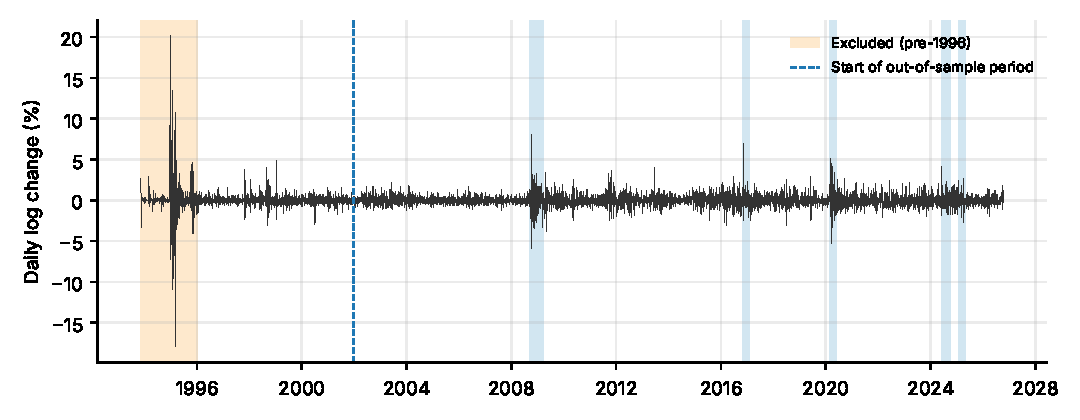
\includegraphics[width=\linewidth]{figures/fig_returns.pdf}
\caption{Daily USD/MXN log changes, November 1993 to October 2026. The shaded orange area (pre-1996) is excluded from the main sample; blue bands mark the stress episodes analysed in Section~\ref{sec:results}; the dashed line marks the first out-of-sample forecast.}\label{fig:returns}
\end{figure}

\section{Models and estimation}\label{sec:models}

\subsection{Models with independent increments}

If the log exchange rate follows a Lévy process $X_t$, daily returns are independent and identically distributed with characteristic function $\E[e^{iuX_1}] = \exp\{\psi(u)\}$. We consider four cases.

\paragraph{Gaussian and Student-$t$.} Brownian motion with drift gives $r_t \sim N(\mu,\sigma^2)$. As a heavy-tailed benchmark without jumps we use a location-scale Student-$t$ distribution with $\nu$ degrees of freedom.

\paragraph{Merton.} The Merton process is $X_t = bt + \sigma W_t + \sum_{j=1}^{N_t} Y_j$, where $N_t$ is a Poisson process with intensity $\lambda$ and $Y_j \sim N(\mu_J,\delta_J^2)$ are independent jump sizes. Conditioning on the number of jumps gives the exact daily density
\begin{equation}\label{eq:merton}
f(r) = \sum_{k=0}^{\infty} \frac{e^{-\lambda}\lambda^k}{k!}\,\phi\!\left(r;\, b + k\mu_J,\; \sigma^2 + k\delta_J^2\right),
\end{equation}
with $\phi(\cdot\,; m, v)$ the normal density with mean $m$ and variance $v$. We truncate the sum at $k=30$; for the estimated intensities the omitted Poisson mass is below machine precision. A positive $\mu_J$ makes large depreciations more likely than large appreciations.

\paragraph{Kou.} In the double-exponential model \citep{kou2002}, a jump is upward with probability $p$ and size $\sim \mathrm{Exp}(\eta_+)$, and downward with probability $1-p$ and size $\sim \mathrm{Exp}(\eta_-)$. We allow at most one jump per day, occurring with probability $q$ \citep{balltorous1983}. The density is then a mixture of a normal and two exponentially modified Gaussian densities,
\begin{equation}\label{eq:kou}
f(r) = (1-q)\,\phi(r; b,\sigma^2) + q\,p\,g_+(r) + q\,(1-p)\,g_-(r),
\end{equation}
where $g_+(r) = \eta_+ \exp\{\eta_+(b-r) + \eta_+^2\sigma^2/2\}\,\Phi\big((r-b-\eta_+\sigma^2)/\sigma\big)$, $\Phi$ is the standard normal distribution function, and $g_-$ is the mirror image with rate $\eta_-$. The distribution functions of both models are available in closed form, which we use for quantiles and probability integral transforms.

\subsection{GARCH models}

To allow volatility clustering, we write $r_t = \mu + \sqrt{h_t}\, z_t + J_t$, where $J_t$ is a jump term (absent in the GARCH-$t$ and GARCH-skew-$t$ models) and
\begin{equation}\label{eq:garch}
h_t = \omega + \alpha\, \varepsilon_{t-1}^2 + \beta\, h_{t-1}, \qquad \varepsilon_t = r_t - \E_{t-1}[r_t],
\end{equation}
with $\omega>0$, $\alpha,\beta\ge 0$ and $\alpha+\beta<1$. The recursion uses the total innovation, so a jump raises volatility on subsequent days, in the spirit of the ARCH-jump model of \citet{jorion1988}. The four specifications are:
\begin{itemize}
\item \textbf{GARCH-$t$}: $z_t$ follows a Student-$t$ distribution standardised to unit variance \citep{bollerslev1987}.
\item \textbf{GARCH-skew-$t$}: $z_t$ follows the standardised skewed-$t$ distribution of \citet{hansen1994}, with tail parameter $\nu$ and asymmetry parameter $\varsigma\in(-1,1)$; $\varsigma>0$ gives a heavier right (depreciation) tail.
\item \textbf{GARCH-Merton}: $z_t\sim N(0,1)$ and $J_t$ is a compound Poisson sum with intensity $\lambda$ and $N(\mu_J,\delta_J^2)$ jumps; the conditional density is \eqref{eq:merton} with $\sigma^2$ replaced by $h_t$.
\item \textbf{GARCH-Kou}: $z_t\sim N(0,1)$ and $J_t$ is a Kou jump; the conditional density is \eqref{eq:kou} with $\sigma^2$ replaced by $h_t$.
\end{itemize}
The variance recursion starts from the sample variance of the estimation window.

\subsection{Estimation}

All parameters are estimated by maximum likelihood with the L-BFGS-B algorithm under box constraints, from several deterministic starting values; we keep the solution with the highest likelihood. Standard errors are robust quasi-maximum-likelihood (sandwich) standard errors \citep{bollerslevwooldridge1992} computed from numerical derivatives. Estimates are physical-measure parameters of the return distribution and should not be read as risk-neutral parameters implied by option prices.

Table~\ref{tab:insample} reports full-sample estimates. Volatility is highly persistent ($\alpha+\beta = \gtPersist$ in the GARCH-$t$ model). The skewed-$t$ GARCH model raises the log-likelihood by \llGainSkew{} points over GARCH-$t$ with one extra parameter, and its asymmetry parameter $\varsigma = \gsLam$ (s.e.\ \gsLamSe) confirms a heavier depreciation tail. Adding jumps to a Gaussian GARCH model is much less effective: the GARCH-Merton log-likelihood is \llLossMerton{} points \emph{below} that of GARCH-$t$ despite two extra parameters, and GARCH-Kou gains only \llGainKou{} points with three extra parameters. The jump estimates themselves are revealing. The GARCH-Merton intensity $\hat\lambda=\gmLambda$ implies a jump every \gmJumpEvery{} trading days on average, far more often than any reasonable count of discontinuous news; and the GARCH-Kou model estimates that \gkPup{} of jumps are depreciations, with similar mean sizes in both directions (\gkMeanUp\% and \gkMeanDn\%). The jump components act as a frequent, asymmetric mixture that thickens the right tail, rather than as rare discontinuities.

\begin{table}[t]
\centering\small
\caption{Full-sample maximum-likelihood estimates, January 1996 -- October 2026 ($n=\nMain$). Robust QMLE standard errors in parentheses. $k$: number of parameters.}\label{tab:insample}
\resizebox{\linewidth}{!}{\begin{tabular}{lrrrrp{0.45\linewidth}}
\toprule
Model & $k$ & log $L$ & AIC & BIC & Estimates (robust s.e.) \\
\midrule
Gaussian & 2 & -8,067.5 & 16,139.1 & 16,153.0 & \parbox[t]{0.45\linewidth}{\raggedright\scriptsize $\mu$=0.011 (0.008), $\sigma$=0.688 (0.014)} \\
Student-t & 3 & -7,226.3 & 14,458.7 & 14,479.6 & \parbox[t]{0.45\linewidth}{\raggedright\scriptsize $\nu$=3.365 (0.138), $\mu$=-0.019 (0.006), $s$=0.450 (0.007)} \\
Merton & 5 & -7,246.6 & 14,503.2 & 14,538.0 & \parbox[t]{0.45\linewidth}{\raggedright\scriptsize $b$=-0.044 (0.009), $\sigma$=0.419 (0.020), $\lambda$=0.306 (0.066), $\mu_J$=0.181 (0.035), $\delta_J$=0.934 (0.088)} \\
Kou & 6 & -7,218.8 & 14,449.5 & 14,491.2 & \parbox[t]{0.45\linewidth}{\raggedright\scriptsize $b$=-0.081 (0.018), $\sigma$=0.381 (0.022), $q$=0.473 (0.072), $p$=0.653 (0.047), $\eta_+$=1.687 (0.115), $\eta_-$=1.811 (0.177)} \\
GARCH-t & 5 & -6,591.9 & 13,193.8 & 13,228.5 & \parbox[t]{0.45\linewidth}{\raggedright\scriptsize $\mu$=-0.019 (0.006), $\omega$=0.009 (0.002), $\alpha$=0.128 (0.017), $\beta$=0.859 (0.018), $\nu$=6.586 (0.480)} \\
GARCH-skew-t & 6 & -6,546.8 & 13,105.5 & 13,147.2 & \parbox[t]{0.45\linewidth}{\raggedright\scriptsize $\mu$=-0.004 (0.006), $\omega$=0.008 (0.002), $\alpha$=0.120 (0.016), $\beta$=0.866 (0.018), $\nu$=7.035 (0.527), $\varsigma$=0.154 (0.016)} \\
GARCH-Merton & 7 & -6,602.7 & 13,219.5 & 13,268.2 & \parbox[t]{0.45\linewidth}{\raggedright\scriptsize $\mu$=-0.042 (0.010), $\omega$=0.004 (0.002), $\alpha$=0.108 (0.016), $\beta$=0.851 (0.023), $\lambda$=0.135 (0.051), $\mu_J$=0.304 (0.072), $\delta_J$=0.706 (0.113)} \\
GARCH-Kou & 8 & -6,591.5 & 13,199.0 & 13,254.6 & \parbox[t]{0.45\linewidth}{\raggedright\scriptsize $\mu$=-0.068 (0.019), $\omega$=0.003 (0.002), $\alpha$=0.106 (0.016), $\beta$=0.855 (0.024), $q$=0.223 (0.082), $p$=0.835 (0.069), $\eta_+$=2.195 (0.339), $\eta_-$=2.172 (0.512)} \\
\bottomrule
\end{tabular}
}
\end{table}

\section{Forecasting design and evaluation}\label{sec:eval}

\paragraph{Rolling forecasts.} Each model is estimated on a rolling window of \windowLen{} returns (about six years) and re-estimated every \refitEvery{} returns (about one month). Between re-estimations, parameters are fixed, while GARCH variances are updated daily with observed returns, so the forecast for day $t$ uses information up to $t-1$ only. The first forecast is for \oosStart{}, giving \oosN{} out-of-sample days that cover all five stress episodes. To reduce the cost of repeated estimation, each re-estimation starts from the previous estimate and one default value, and every twelfth uses the full set of starting values.

\paragraph{Risk measures.} We focus on the upper tail, which measures the risk of peso depreciation for anyone who must buy dollars. For $\alpha\in\{0.95,0.99\}$, $\VaR_{\alpha,t} = F_{t}^{-1}(\alpha)$ and $\ES_{\alpha,t} = (1-\alpha)^{-1}\int_\alpha^1 F_t^{-1}(u)\,du$ \citep{rockafellaruryasev2002}, where $F_t$ is the one-step predictive distribution. Quantiles are computed by bisection on the closed-form distribution functions, and ES by numerical integration of the survival function.

\paragraph{Scoring.} Density forecasts are compared with the negative log score $-\log f_t(r_t)$, a strictly proper scoring rule \citep{gneitingraftery2007}. VaR and ES are compared jointly with the FZ0 loss of \citet{pattonziegelchen2019}, which is strictly consistent for the pair \citep{fisslerziegel2016}. Applied to the upper tail through $x_t=-r_t$, $v_t=-\VaR_{\alpha,t}$, $e_t=-\ES_{\alpha,t}$ and $a=1-\alpha$,
\begin{equation}
L_{\mathrm{FZ0}}(x_t, v_t, e_t) = -\frac{1}{a\,e_t}\,\mathbf{1}\{x_t\le v_t\}\,(v_t-x_t) + \frac{v_t}{e_t} + \log(-e_t) - 1.
\end{equation}

\paragraph{Backtests.} For each model and level we report the number of VaR exceedances, the unconditional coverage test of \citet{kupiec1995} (UC) and the conditional coverage test of \citet{christoffersen1998} (CC). Expected Shortfall is backtested with the unconditional test of \citet{duescanciano2017}: with $u_t = 1-F_t(r_t)$, the cumulative violation $H_t = (a-u_t)a^{-1}\mathbf{1}\{u_t\le a\}$ has mean $a/2$ and variance $a(1/3-a/4)$ under correct specification.

\paragraph{Model comparison.} Pairwise Diebold--Mariano tests compare each model with GARCH-$t$, using Newey--West standard errors with 10 lags \citep{dieboldmariano1995,neweywest1987}. The Model Confidence Set (MCS) of \citet{hansenlundenason2011} identifies the models that cannot be rejected as best at the 10\% level, using the range statistic and a stationary block bootstrap \citep{politisromano1994} with \mcsReps{} replications and average block length 10.

\section{Empirical results}\label{sec:results}

\subsection{Calibration}

Table~\ref{tab:oos} reports the coverage and ES backtests. With \oosN{} forecasts, \expNinetyFive{} and \expNinetyNine{} exceedances are expected at the 95\% and 99\% levels. We see three patterns.

First, every model with independent increments fails the conditional coverage test at both levels ($p<0.001$). Their exceedances arrive in clusters during turbulent periods, which a constant-volatility model cannot anticipate. The i.i.d.\ Merton and Kou models obtain nearly correct \emph{unconditional} 99\% coverage (\excNNMerton{} and \excNNKou{} exceedances) and pass the unconditional ES test, but only because their constant VaR is wide enough on average. The count is right, but the timing is not.

Second, the symmetric GARCH-$t$ model under-predicts depreciation risk. It records \excNNGarchT{} exceedances of the 99\% VaR and \excNFGarchT{} of the 95\% VaR, and fails all three tests at both levels.

Third, three models with an asymmetric tail pass all 99\% tests: GARCH-skew-$t$ (\excNNGarchSkewT{} exceedances, CC $p=\pccNNGarchSkewT$, ES $p=\puesNNGarchSkewT$), GARCH-Kou (\excNNGarchKou; CC $p=\pccNNGarchKou$) and GARCH-Merton (\excNNGarchMerton; CC $p=\pccNNGarchMerton$). At the 95\% level, GARCH-skew-$t$ is the only GARCH model that passes the unconditional coverage and ES tests, and all models fail conditional coverage, a reminder that a GARCH(1,1) recursion does not capture all the clustering of moderate depreciations. The probability integral transforms in Figure~\ref{fig:pit} agree: GARCH-$t$ places too little mass in the extreme right tail, whereas the asymmetric models produce nearly uniform transforms.

\begin{table}[t]
\centering\small
\caption{Out-of-sample calibration, \oosStart{} -- \sampleEnd{} ($n=\oosN$). NLS: mean negative log score. Exc.: VaR exceedances (expected \expNinetyFive{} and \expNinetyNine). UC: Kupiec unconditional coverage $p$-value. CC: Christoffersen conditional coverage $p$-value. ES: Du--Escanciano unconditional ES backtest $p$-value.}\label{tab:oos}
\resizebox{\linewidth}{!}{\begin{tabular}{lrrrrrrrrr}
\toprule
Model & NLS & \multicolumn{4}{c}{95\% upper tail} & \multicolumn{4}{c}{99\% upper tail} \\\cmidrule(lr){3-6}\cmidrule(lr){7-10} & & Exc. & UC & CC & ES & Exc. & UC & CC & ES \\
\midrule
Gaussian & 1.1136 & 311 & 0.991 & $<$0.001 & $<$0.001 & 123 & $<$0.001 & $<$0.001 & $<$0.001 \\
Student-t & 0.9867 & 416 & $<$0.001 & $<$0.001 & $<$0.001 & 90 & $<$0.001 & $<$0.001 & $<$0.001 \\
Merton & 1.0048 & 345 & 0.053 & $<$0.001 & 0.627 & 54 & 0.283 & $<$0.001 & 0.765 \\
Kou & 0.9948 & 346 & 0.047 & $<$0.001 & 0.605 & 55 & 0.347 & $<$0.001 & 0.673 \\
GARCH-t & 0.9036 & 406 & $<$0.001 & $<$0.001 & $<$0.001 & 96 & $<$0.001 & $<$0.001 & $<$0.001 \\
GARCH-skew-t & 0.8994 & 338 & 0.124 & 0.009 & 0.156 & 74 & 0.146 & 0.344 & 0.707 \\
GARCH-Merton & 0.9069 & 369 & 0.001 & $<$0.001 & 0.002 & 78 & 0.053 & 0.101 & 0.123 \\
GARCH-Kou & 0.9059 & 360 & 0.006 & $<$0.001 & 0.005 & 73 & 0.182 & 0.232 & 0.333 \\
\bottomrule
\end{tabular}
}
\end{table}

\begin{figure}[t]
\centering
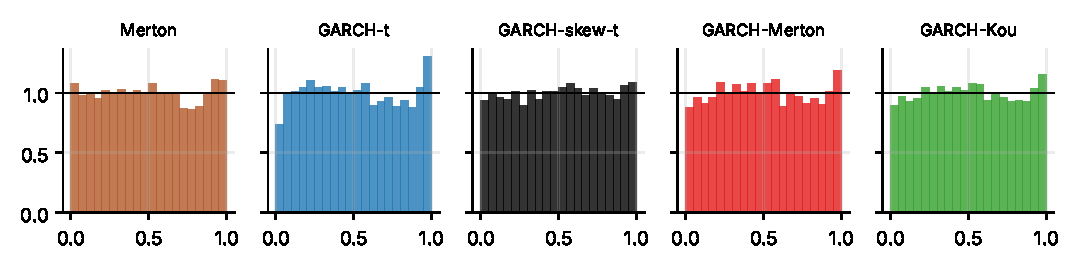
\includegraphics[width=\linewidth]{figures/fig_pit.pdf}
\caption{Histograms of out-of-sample probability integral transforms $F_t(r_t)$. A correctly specified model gives a uniform histogram (horizontal line). Mass near 1 corresponds to depreciations larger than predicted.}\label{fig:pit}
\end{figure}

\subsection{Scores and model comparison}

Calibration tests can accept several models; scoring rules rank them. Table~\ref{tab:compare} shows that volatility clustering is by far the most important feature. Every model with independent increments has a significantly worse log score than GARCH-$t$ (Diebold--Mariano $t$-statistics between \dmtNlsGaussian{} and \dmtNlsStudentT) and a significantly worse FZ0 loss.

Among GARCH models, jumps do not improve the scores. GARCH-Merton and GARCH-Kou have slightly \emph{higher} log scores than GARCH-$t$ (DM $p=\dmpNlsGarchMerton$ and $\dmpNlsGarchKou$) and statistically indistinguishable FZ0 losses at both levels. They fix coverage at 99\% but do not produce more accurate VaR--ES pairs. In contrast, GARCH-skew-$t$ improves on GARCH-$t$ for the log score ($t=\dmtNlsGarchSkewT$, $p=\dmpNlsGarchSkewT$) and the 95\% FZ0 loss ($t=\dmtFzNineFiveGarchSkewT$, $p=\dmpFzNineFiveGarchSkewT$), with a gain of borderline significance at 99\% ($p=\dmpFzNineNineGarchSkewT$). It is the only model in the 10\% MCS for the log score and the 95\% FZ0 loss. For the 99\% FZ0 loss, which is based on few observations, the MCS retains the four GARCH models but GARCH-skew-$t$ ranks first.

\begin{table}[t]
\centering\small
\caption{Out-of-sample scores. Mean: average loss (lower is better). DM $t$: Diebold--Mariano statistic for the loss difference with GARCH-$t$ (negative: better than GARCH-$t$), Newey--West standard errors with 10 lags. MCS $p$: Model Confidence Set $p$-value; bold: model in the 10\% MCS.}\label{tab:compare}
\resizebox{\linewidth}{!}{\begin{tabular}{lrrrrrrrrr}
\toprule
Model & \multicolumn{3}{c}{Negative log score} & \multicolumn{3}{c}{FZ0 loss, 95\%} & \multicolumn{3}{c}{FZ0 loss, 99\%} \\\cmidrule(lr){2-4}\cmidrule(lr){5-7}\cmidrule(lr){8-10} & Mean & DM $t$ & MCS $p$ & Mean & DM $t$ & MCS $p$ & Mean & DM $t$ & MCS $p$ \\
\midrule
Gaussian & 1.1136 & +2.94 & 0.016 & 0.5944 & +3.05 & 0.017 & 1.4078 & +2.55 & 0.080 \\
Student-t & 0.9867 & +6.37 & 0.000 & 0.6098 & +3.30 & 0.015 & 1.2578 & +2.42 & 0.089 \\
Merton & 1.0048 & +4.49 & 0.002 & 0.5906 & +3.45 & 0.011 & 1.2204 & +2.55 & 0.063 \\
Kou & 0.9948 & +5.20 & 0.000 & 0.5865 & +3.40 & 0.012 & 1.1845 & +2.58 & 0.055 \\
GARCH-t & 0.9036 & -- & 0.016 & 0.3838 & -- & 0.034 & 0.7697 & -- & \textbf{0.106} \\
GARCH-skew-t & 0.8994 & -2.91 & \textbf{1.000} & 0.3717 & -2.60 & \textbf{1.000} & 0.7473 & -1.87 & \textbf{1.000} \\
GARCH-Merton & 0.9069 & +1.29 & 0.016 & 0.3828 & -0.18 & 0.049 & 0.7916 & +1.06 & \textbf{0.106} \\
GARCH-Kou & 0.9059 & +1.00 & 0.016 & 0.3835 & -0.06 & 0.049 & 0.7886 & +0.88 & \textbf{0.106} \\
\bottomrule
\end{tabular}
}
\end{table}

Figure~\ref{fig:cumloss} shows how these differences accumulate. The skewed-$t$ model gains steadily against GARCH-$t$, with no single episode responsible. The jump models track GARCH-$t$ closely until the 2008 crisis and fall behind gradually afterwards; their losses are spread over many ordinary days rather than concentrated in the stress episodes.

\begin{figure}[t]
\centering
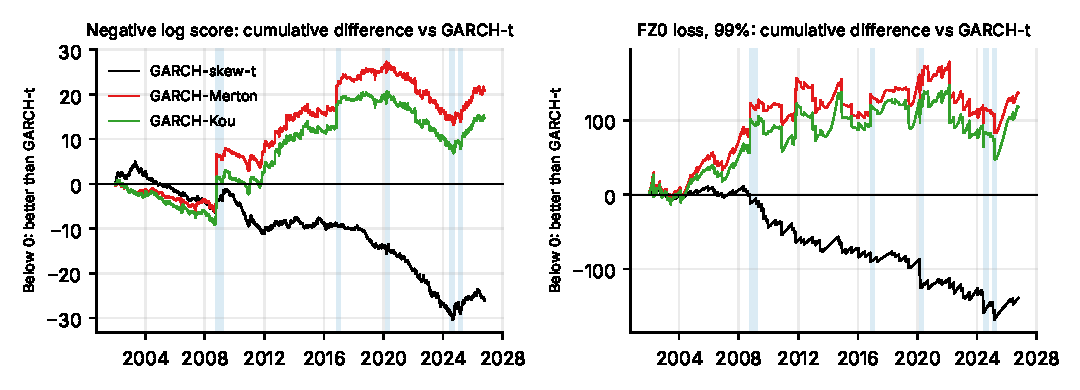
\includegraphics[width=\linewidth]{figures/fig_cumloss.pdf}
\caption{Cumulative out-of-sample loss differences relative to GARCH-$t$. A declining line indicates that the model outperforms GARCH-$t$. Blue bands mark stress episodes.}\label{fig:cumloss}
\end{figure}

\subsection{Stress episodes and time variation}

Table~\ref{tab:events} counts 99\% VaR exceedances in the five stress episodes. Models with independent increments fail badly in the 2008 crisis and the COVID-19 shock (for example, 17--27 exceedances in 135 days during the financial crisis, against 1.35 expected), because their VaR does not respond to the rise in volatility (Figure~\ref{fig:var}). All GARCH models adapt within days and have similar counts in each episode; the episodes do not discriminate between jumps and asymmetry.

\begin{table}[t]
\centering\small
\caption{Exceedances of the 99\% VaR during stress episodes. Days: out-of-sample days in the episode. Max $r_t$: largest daily depreciation (\%). Best NLS: model with the lowest mean negative log score in the episode.}\label{tab:events}
\resizebox{\linewidth}{!}{\begin{tabular}{p{0.24\linewidth}rrrrrrrrrrl}
\toprule
Episode & Days & Max $r_t$ & Gauss & $t$ & Merton & Kou & G-$t$ & G-skew-$t$ & G-Merton & G-Kou & Best NLS \\
\midrule
Global financial crisis & 135 & 8.11 & 27 & 26 & 19 & 17 & 3 & 3 & 4 & 4 & GARCH-t \\
U.S. election 2016 & 60 & 7.01 & 5 & 3 & 3 & 3 & 1 & 1 & 1 & 1 & GARCH-skew-t \\
COVID-19 shock & 70 & 5.15 & 14 & 11 & 10 & 10 & 4 & 4 & 4 & 5 & GARCH-skew-t \\
Mexican election and judicial reform & 83 & 4.16 & 4 & 3 & 2 & 2 & 2 & 2 & 2 & 2 & GARCH-Kou \\
U.S. tariff announcements 2025 & 71 & 2.67 & 2 & 2 & 1 & 1 & 2 & 2 & 2 & 2 & Kou \\
\bottomrule
\end{tabular}
}
\end{table}

\begin{figure}[t]
\centering
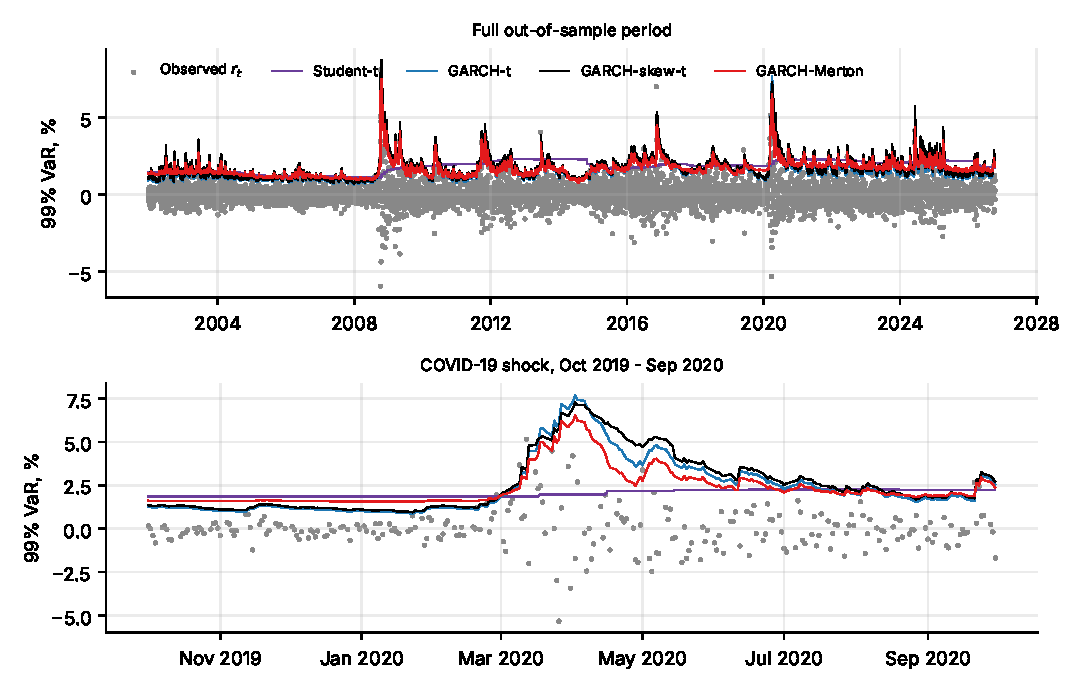
\includegraphics[width=\linewidth]{figures/fig_var.pdf}
\caption{One-day 99\% VaR forecasts and observed returns. Top: full out-of-sample period. Bottom: October 2019 -- September 2020.}\label{fig:var}
\end{figure}

The rolling jump estimates are unstable (Figure~\ref{fig:params}). The GARCH-Merton intensity ranges from almost zero to more than one jump every two days, and jump sizes change abruptly between neighbouring windows. The share of upward jumps in the GARCH-Kou model stays above one half in almost every window, often close to one. This instability is consistent with the large sampling error of jump parameters documented in Section~\ref{sec:mc}; the jump parameters are better interpreted as flexible shape parameters than as a structural description of news arrival.

\begin{figure}[t]
\centering
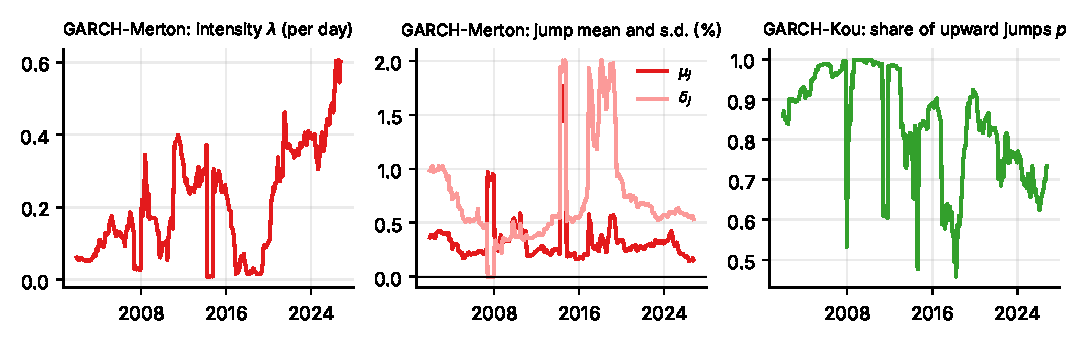
\includegraphics[width=\linewidth]{figures/fig_parameters.pdf}
\caption{Rolling estimates of jump parameters at each monthly re-estimation (window of \windowLen{} returns).}\label{fig:params}
\end{figure}

\section{Application: an importer's currency risk}\label{sec:app}

To translate these differences into money, consider a Mexican importer that owes USD 1 million and holds pesos. If the peso depreciates by $r_t$ percent, the peso cost of the payable rises by $10^6\, S_{t-1}(e^{r_t/100}-1)$. Table~\ref{tab:app} reports the average one-day 99\% VaR and ES of this exposure, the number of days on which the loss exceeded the VaR, and the total loss in excess of the ES forecast, summed over the out-of-sample period.

\begin{table}[t]
\centering\small
\caption{One-day risk of a USD 1 million payable, in thousands of Mexican pesos, \oosStart{} -- \sampleEnd. Mean excess: average loss in excess of VaR on breach days. Shortfall beyond ES: sum over all days of losses in excess of the ES forecast.}\label{tab:app}
\begin{tabular}{lrrrrr}
\toprule
Model & Mean VaR$_{99}$ & Mean ES$_{99}$ & Breaches & Mean excess & Shortfall beyond ES \\
\midrule
Gaussian & 255.8 & 293.1 & 123 & 128.8 & 12,096 \\
Student-t & 289.4 & 417.8 & 90 & 143.0 & 6,996 \\
Merton & 332.0 & 419.6 & 54 & 190.3 & 6,268 \\
Kou & 326.0 & 422.9 & 55 & 185.1 & 6,194 \\
GARCH-t & 262.1 & 329.1 & 96 & 73.8 & 3,351 \\
GARCH-skew-t & 283.8 & 356.6 & 74 & 74.1 & 2,776 \\
GARCH-Merton & 269.9 & 337.4 & 78 & 87.1 & 3,794 \\
GARCH-Kou & 273.2 & 343.2 & 73 & 89.8 & 3,671 \\
\bottomrule
\end{tabular}

\end{table}

Apart from the Gaussian model, the models with independent increments demand the largest average ES buffers (about MXN \appEsMerton{} thousand for Merton), yet leave the largest uncovered losses, because their buffers are too large in calm periods and too small in crises. Among GARCH models, the skewed-$t$ model asks for a moderately larger buffer than GARCH-$t$ (MXN \appEsGarchSkewT{} versus \appEsGarchT{} thousand on average) and in exchange has far fewer breaches (\excNNGarchSkewT{} against \excNNGarchT) and the smallest total shortfall beyond ES of all models (MXN \appShortGarchSkewT{} thousand, against \appShortGarchT{} thousand for GARCH-$t$). The jump models also reduce the number of breaches, but the losses on breach days are larger, and their total shortfall beyond ES (MXN \appShortGarchMerton{} and \appShortGarchKou{} thousand) exceeds even that of GARCH-$t$. For a treasurer, the asymmetric GARCH model buys better protection against depreciation at a modest cost in average reserves.

\section{Robustness}\label{sec:robust}

Table~\ref{tab:robust} repeats the evaluation for three alternative designs, always on the same \oosN{} out-of-sample days: a shorter rolling window of 1,000 returns; weekly instead of monthly re-estimation; and an expanding window that starts in November 1993 and therefore contains the end of the exchange-rate band and the 1994--95 crisis, re-estimated every 63 returns. The last design is close to that of an earlier version of this study.

\begin{table}[t]
\centering\small
\caption{Robustness of the out-of-sample comparison to the estimation design. NLS: mean negative log score (bold: lowest). Exc.\ 99\%: exceedances of the 99\% VaR (expected \expNinetyNine). FZ0 99\%: mean joint VaR--ES loss at the 99\% level.}\label{tab:robust}
\resizebox{\linewidth}{!}{\begin{tabular}{lrrrrrrrr}
\toprule
 & Gauss & $t$ & Merton & Kou & G-$t$ & G-skew-$t$ & G-Merton & G-Kou \\
\midrule
\multicolumn{9}{l}{\textit{Rolling 1500, refit 21}} \\
\quad NLS & 1.1136 & 0.9867 & 1.0048 & 0.9948 & 0.9036 & \textbf{0.8994} & 0.9069 & 0.9059 \\
\quad Exc. 99\% & 123 & 90 & 54 & 55 & 96 & 74 & 78 & 73 \\
\quad FZ0 99\% & 1.408 & 1.258 & 1.220 & 1.185 & 0.770 & 0.747 & 0.792 & 0.789 \\
\multicolumn{9}{l}{\textit{Rolling 1000, refit 21}} \\
\quad NLS & 1.1268 & 0.9881 & 1.0359 & 0.9943 & 0.9049 & \textbf{0.9011} & 0.9092 & 0.9065 \\
\quad Exc. 99\% & 128 & 83 & 62 & 62 & 98 & 79 & 79 & 68 \\
\quad FZ0 99\% & 1.443 & 1.338 & 1.260 & 1.231 & 0.774 & 0.756 & 0.796 & 0.791 \\
\multicolumn{9}{l}{\textit{Rolling 1500, refit 5}} \\
\quad NLS & 1.0999 & 0.9824 & 0.9951 & 0.9853 & 0.9032 & \textbf{0.8987} & 0.9062 & 0.9053 \\
\quad Exc. 99\% & 122 & 89 & 53 & 55 & 97 & 74 & 77 & 72 \\
\quad FZ0 99\% & 1.366 & 1.216 & 1.160 & 1.140 & 0.768 & 0.744 & 0.785 & 0.782 \\
\multicolumn{9}{l}{\textit{Expanding from Nov 1993, refit 63}} \\
\quad NLS & 1.1826 & 0.9966 & 1.0145 & 1.0071 & 0.9113 & \textbf{0.9060} & 0.9130 & 0.9116 \\
\quad Exc. 99\% & 45 & 51 & 16 & 23 & 97 & 68 & 70 & 72 \\
\quad FZ0 99\% & 1.170 & 1.168 & 1.361 & 1.287 & 0.772 & 0.757 & 0.814 & 0.812 \\
\bottomrule
\end{tabular}
}
\end{table}

The ranking of the GARCH models does not depend on the window length or the re-estimation frequency. In every design GARCH-skew-$t$ has the lowest log score and the lowest 99\% FZ0 loss, GARCH-$t$ has too many 99\% exceedances (between \excNNGarchT{} and \robExcWindowOneZeroZeroZeroGarchT), and the jump-GARCH models reduce the number of exceedances without improving the scores.

Including the 1994--95 observations changes the results for the models with independent increments, and reproduces the problem that motivated this redesign. Estimated on the expanding sample, the i.i.d.\ Merton model fits its jump component to the crisis, with jump standard deviations of up to 3\%, and produces a 99\% VaR that is exceeded only \robExcExpandingOneNineNineThreeMerton{} times, against \expNinetyNine{} expected; at the same time its 95\% VaR is exceeded far too often. So a 99\% VaR that looks conservative is not evidence of good calibration here. It comes from one historical episode. GARCH models are much less affected, because their conditional variance absorbs the crisis, and their ranking is unchanged.


\section{Monte Carlo evidence}\label{sec:mc}

Can daily data distinguish jumps from asymmetric heavy tails, and how should the empirical ranking be read? To answer these questions we simulate from five data-generating processes (DGPs) whose parameters equal the full-sample estimates in Table~\ref{tab:insample}: Gaussian, i.i.d.\ Merton, GARCH-$t$, GARCH-skew-$t$ and GARCH-Merton. In each of \mcReps{} replications per DGP we simulate \mcTrain{}~+~\mcTest{} returns, estimate all eight models on the first \mcTrain{} observations (the length of the rolling window) and evaluate one-step-ahead forecasts on the last \mcTest{}, with GARCH variances filtered from past simulated returns. Table~\ref{tab:mc} reports mean negative log scores, 99\% VaR exceedance rates and the share of replications in which each model has the best score.

\begin{table}[t]
\centering\small
\caption{Monte Carlo results: \mcReps{} replications per DGP, \mcTrain{} estimation and \mcTest{} evaluation observations. First row of each block: mean negative log score (bold: lowest). Second row: mean 99\% VaR exceedance rate in \% (nominal 1\%). Third row: share of replications in which the model has the lowest log score.}\label{tab:mc}
\resizebox{\linewidth}{!}{\begin{tabular}{lrrrrrrrr}
\toprule
DGP & Gauss & $t$ & Merton & Kou & G-$t$ & G-skew-$t$ & G-Merton & G-Kou \\
\midrule
Gaussian & \textbf{1.0477} & 1.0478 & 1.0481 & 1.0479 & 1.0480 & 1.0484 & 1.0482 & 1.0481 \\
\quad 99\% exc. (\%) & 1.00 & 0.97 & 1.00 & 1.00 & 0.97 & 0.97 & 1.01 & 1.01 \\
\quad Best NLS (\%) & 24 & 12 & 16 & 2 & 14 & 16 & 8 & 10 \\
\midrule
Merton & 1.0232 & 0.9474 & \textbf{0.9420} & 0.9424 & 0.9477 & 0.9452 & 0.9423 & 0.9427 \\
\quad 99\% exc. (\%) & 2.50 & 1.55 & 1.01 & 1.00 & 1.54 & 1.13 & 1.01 & 1.00 \\
\quad Best NLS (\%) & 0 & 4 & 30 & 16 & 3 & 7 & 26 & 13 \\
\midrule
GARCH-t & 1.1707 & 0.9765 & 0.9902 & 0.9829 & \textbf{0.8644} & 0.8648 & 0.8721 & 0.8715 \\
\quad 99\% exc. (\%) & 1.96 & 1.27 & 1.19 & 1.19 & 0.98 & 1.00 & 1.14 & 1.13 \\
\quad Best NLS (\%) & 0 & 0 & 0 & 0 & 50 & 34 & 8 & 8 \\
\midrule
GARCH-skew-t & 1.1582 & 0.9586 & 0.9732 & 0.9632 & 0.8472 & \textbf{0.8412} & 0.8519 & 0.8497 \\
\quad 99\% exc. (\%) & 2.38 & 1.69 & 1.35 & 1.33 & 1.51 & 1.04 & 1.23 & 1.18 \\
\quad Best NLS (\%) & 0 & 0 & 0 & 0 & 11 & 77 & 6 & 6 \\
\midrule
GARCH-Merton & 0.9890 & 0.9415 & 0.9403 & 0.9403 & 0.8704 & 0.8682 & 0.8637 & \textbf{0.8635} \\
\quad 99\% exc. (\%) & 2.34 & 1.58 & 1.24 & 1.15 & 1.51 & 1.26 & 1.08 & 1.12 \\
\quad Best NLS (\%) & 0 & 0 & 0 & 0 & 4 & 8 & 44 & 44 \\
\bottomrule
\end{tabular}
}
\end{table}

We draw three conclusions. First, the mechanism is identifiable at this sample size. The Bayesian information criterion selects the true model in \mcBicGarchMertonGarchMerton\% of GARCH-Merton samples, \mcBicGarchSkewTGarchSkewT\% of GARCH-skew-$t$ samples and \mcBicGarchTGarchT\% of GARCH-$t$ samples. Out of sample, the correctly specified class also has the lowest mean score for every DGP; under the GARCH-Merton DGP the two jump-GARCH models are essentially tied, because a Kou mixture approximates a Merton mixture well.

Second, the simulations show how to read the empirical evidence. When data come from the GARCH-Merton process, the jump models beat GARCH-$t$ (mean scores \mcNlsGarchMertonGarchMerton{} and \mcNlsGarchMertonGarchT) and the skewed-$t$ model lies in between (\mcNlsGarchMertonGarchSkewT). When data come from the GARCH-skew-$t$ process, the order is skewed-$t$ first (\mcNlsGarchSkewTGarchSkewT), GARCH-$t$ second (\mcNlsGarchSkewTGarchT) and the jump models last (\mcNlsGarchSkewTGarchMerton{} and \mcNlsGarchSkewTGarchKou). The empirical ranking in Table~\ref{tab:compare}, with the skewed-$t$ model better and the jump models worse than GARCH-$t$, matches the second pattern and not the first. Coverage agrees as well: under the skewed-$t$ DGP the 99\% VaR of the GARCH-$t$ model is exceeded on \mcExcGarchSkewTGarchT\% of days, close to the \rateNNGarchT\% observed for the peso, and the jump models reduce this to \mcExcGarchSkewTGarchKou--\mcExcGarchSkewTGarchMerton\%. The partial repair of coverage by jump models is therefore exactly what one would expect if the peso had asymmetric tails and no jumps at all.

Third, even when jumps are present, their parameters are estimated imprecisely. Under the GARCH-Merton DGP, with true intensity $\lambda=\mcTrueLambda$, the root mean squared error of $\hat\lambda$ is \mcRmseLambda{} and 90\% of the estimates lie between \mcLoLambda{} and \mcHiLambda; for the mean jump size ($\mu_J=\mcTrueMuj$) the root mean squared error is \mcRmseMuj. The instability of the rolling jump estimates in Figure~\ref{fig:params} is of the size that sampling error alone would produce. Finally, when data are i.i.d.\ (Gaussian or Merton DGPs), the GARCH models lose very little relative to the true model, so allowing for volatility clustering carries almost no cost.


\section{Conclusions}\label{sec:conclusion}

Lévy jump-diffusion models are a natural way to describe abrupt depreciations of the Mexican peso. Their forecasting value, however, depends on what they are compared with. Against models with independent increments, every model with volatility clustering wins decisively; a jump component cannot substitute for volatility dynamics. Against a symmetric GARCH-$t$ model, adding Merton or Kou jumps corrects the under-prediction of extreme depreciations, but it does so by making the conditional distribution asymmetric: the estimated jumps are frequent and predominantly upward. A GARCH model with skewed-$t$ innovations captures the same asymmetry with fewer parameters, obtains the best density and VaR--ES scores, passes all 99\% backtests and is the only model retained in the Model Confidence Set for the log score. Simulations calibrated to the estimates show that the two mechanisms leave different fingerprints in samples of realistic length, and the fingerprint in the peso data is that of asymmetric heavy tails rather than of compound Poisson jumps. Even when jumps are present, their intensity and size are estimated imprecisely, so economic interpretations of estimated jump parameters should be cautious.

For risk management, the practical lesson is to model the asymmetry of currency risk directly. A symmetric heavy-tailed model, even with volatility clustering, systematically under-states the risk of peso depreciation. The study has limitations that suggest extensions: it uses constant jump intensities and a GARCH(1,1) recursion, a daily frequency at which jumps are hard to identify, and a single currency. Time-varying jump intensities \citep{chanmaheu2002,maheumccurdy2004}, asymmetric volatility responses, intraday data with nonparametric jump tests \citep{leemykland2008}, and option-implied information \citep{bates1996} would be useful extensions, and the same design can be applied to other emerging-market currencies.

\section*{Data and code availability}\label{sec:data-availability}
\phantomsection
The data are the publicly available FRED series DEXMXUS \citep{fred}, downloaded as a CSV file on 24 October 2026 and used without modification. The exact file is included in the replication package. Its SHA-256 checksum is \texttt{\seqsplit{60c8c775e7308e070bad43c65386f7b3855d65410101ba496f15c5df85187738}}, and the code checks it before every run, so any later revision of the FRED series is detected. All results, tables, figures and numbers quoted in the text are produced by the replication package, which runs with a single command (\texttt{python scripts/run\_all.py}) and is available at \url{https://github.com/mferrazfigueiro-eng/mxn-jump-tailrisk}, archived at Zenodo with DOI \href{https://doi.org/10.5281/zenodo.24353202}{10.5281/zenodo.24353202}.

\section*{Statements and declarations}
\noindent\textbf{Funding.} This research received no specific grant from any funding agency.\\
\textbf{Competing interests.} The author declares no competing interests.\\
\textbf{Use of generative AI.} Anthropic Claude was used to assist with writing and debugging the code and with drafting the manuscript. The author designed the study, verified the code, data and results, and takes full responsibility for the content.

\bibliographystyle{unsrtnat}
\bibliography{references}

\end{document}
